\documentclass[aspectratio=169]{../latex_main/tntbeamer}  % you can pass all options of the beamer class, e.g., 'handout' or 'aspectratio=43'
\usepackage{dsfont}
\usepackage{bm}
\usepackage[english]{babel}
\usepackage[T1]{fontenc}
%\usepackage[utf8]{inputenc}
\usepackage{graphicx}
\graphicspath{ {./figures/} }
\usepackage{algorithm}
\usepackage[ruled,vlined,algo2e,linesnumbered]{algorithm2e}
\usepackage{hyperref}
\usepackage{booktabs}
\usepackage{mathtools}

\usepackage{amsmath,amssymb}

\DeclareMathOperator*{\argmax}{arg\,max}
\DeclareMathOperator*{\argmin}{arg\,min}

\usepackage{pgfplots}
\pgfplotsset{compat=1.16}
\usepackage{tikz}
\usetikzlibrary{trees} 
\usetikzlibrary{shapes.geometric}
\usetikzlibrary{positioning,shapes,shadows,arrows,calc,mindmap}
\usetikzlibrary{positioning,fadings,through}
\usetikzlibrary{decorations.pathreplacing}
\usetikzlibrary{intersections}
\pgfdeclarelayer{background}
\pgfdeclarelayer{foreground}
\pgfsetlayers{background,main,foreground}
\tikzstyle{activity}=[rectangle, draw=black, rounded corners, text centered, text width=8em]
\tikzstyle{data}=[rectangle, draw=black, text centered, text width=8em]
\tikzstyle{myarrow}=[->, thick, draw=black]

% Define the layers to draw the diagram
\pgfdeclarelayer{background}
\pgfdeclarelayer{foreground}
\pgfsetlayers{background,main,foreground}

% Requires XeLaTeX or LuaLaTeX
\usepackage{unicode-math}

\usepackage{fontspec}
%\setsansfont{Arial}
\setsansfont{RotisSansSerifStd}[ 
Path=../latex_main/fonts/,
Extension = .otf,
UprightFont = *-Regular,  % or *-Light
BoldFont = *-ExtraBold,  % or *-Bold
ItalicFont = *-Italic
]
\setmonofont{Cascadia Mono}[
Scale=0.8
]

% scale factor adapted; mathrm font added (Benjamin Spitschan @TNT, 2021-06-01)
%\setmathfont[Scale=1.05]{Libertinus Math}
%\setmathrm[Scale=1.05]{Libertinus Math}

% other available math fonts are (not exhaustive)
% Latin Modern Math
% XITS Math
% Libertinus Math
% Asana Math
% Fira Math
% TeX Gyre Pagella Math
% TeX Gyre Bonum Math
% TeX Gyre Schola Math
% TeX Gyre Termes Math

% Literature References
\newcommand{\lit}[2]{\href{#2}{\footnotesize\color{black!60}[#1]}}

%%% Beamer Customization
%----------------------------------------------------------------------
% (Don't) Show sections in frame header. Options: 'sections', 'sections light', empty
\setbeamertemplate{headline}{empty}

% Add header logo for normal frames
\setheaderimage{
	% 
\includegraphics[height=\logoheight]{figures/TNT_darkv4.pdf}
	
\includegraphics[height=\logoheight]{../latex_main/figures/luh_logo_rgb_0_80_155.pdf}
	% 
\includegraphics[height=\logoheight]{figures/logo_tntluh.pdf}
}

% Header logo for title page
\settitleheaderimage{
	% 
\includegraphics[height=\logoheight]{figures/TNT_darkv4.pdf}
	
\includegraphics[height=\logoheight]{../latex_main/figures/luh_logo_rgb_0_80_155.pdf}
	% 
\includegraphics[height=\logoheight]{figures/logo_tntluh.pdf}
}

% Title page: tntdefault 
\setbeamertemplate{title page}[tntdefault]  % or luhstyle
% Add optional title image here
%\addtitlepageimagedefault{
\includegraphics[width=0.65\textwidth]{figures/luh_default_presentation_title_image.jpg}}

% Title page: luhstyle
% \setbeamertemplate{title page}[luhstyle]
% % Add optional title image here
% \addtitlepageimage{
\includegraphics[width=0.75\textwidth]{figures/luh_default_presentation_title_image.jpg}}

\author[Lindauer \& Anand]{Marius Lindauer and Avishek Anand\\[1em]
	
\includegraphics[height=\logoheight]{../latex_main/figures/luh_logo_rgb_0_80_155.pdf}\qquad

\includegraphics[height=\logoheight]{../latex_main/figures/TNT_darkv4}\qquad

\includegraphics[height=\logoheight]{../latex_main/figures/L3S.jpg}	}
\date{Winter Term 2021
}


%%% Custom Packages
%----------------------------------------------------------------------
% Create dummy content
\usepackage{blindtext}

% Adds a frame with the current page layout. Just call \layout inside of a frame.
\usepackage{layout}


\title[Introduction]{iML: Shapley Values}
\subtitle{Background: Game Theory}

%\institute{}


\begin{document}
	
	\maketitle
	
\begin{frame}{Cooperative Games}
\begin{itemize}
  \item In cooperative games, a \alert{set of players $P$} with $P = \{1, \hdots, p\}$ forms a coalition $S \subseteq P$. 
  \pause
  \item A \alert{value function $v(S): 2^{|P|}\mapsto \mathbb{R}$} describes the payout (or gain) achieved by any coalition $\forall S \subseteq P$. The value of the empty coalition must be zero: $v(\emptyset) = 0$.
  \pause
  \item As some players contribute more than others, we are interested to fairly divide the total payout $v(P)$ among the players.
  \pause
  \item We call the \alert{payout per player $\phi_j$}, $j \in P$.
  \pause
  \bigskip
  \item[$\leadsto$] What would be properties of a fair distribution of the payout?
\end{itemize}
\end{frame}


\begin{frame}{Axioms of Fair Payouts}
  One possibility to define \textbf{fair} payouts are the following axioms for a given value function $v$:
  \begin{itemize}
    \item \textbf{Efficiency}: Player contributions add up to the total payout of the game:
      $\sum\nolimits_{j=1}^p\phi_j = v(P)$
    \pause
    \item \textbf{Symmetry}: Players $j\in P$ and $k \in P$ who contribute the same to any coalition get the same payout: \\
      If $v(S \cup \{j\}) = v(S \cup \{k\})$ for all $S \subseteq P - \{j,k\}$, then $\phi_j=\phi_k$
    \pause
    \item \textbf{Dummy / Null Player}: The payout is zero for players who don't contribute to the value of any coalition: \\
      If $v(S \cup \{j\})=v(S)\quad  \forall \quad S \subseteq P - \{j\}$, then $\phi_j=0$
    \pause
    \item \textbf{Additivity}: For a game $v$ with combined payouts $v(S) = v_1(S) + v_2(S)$, the payout is the sum of payouts: $\phi_{j,v} = \phi_{j,v_1} + \phi_{j, v_2}$
  \end{itemize}

  \pause
  Is there an attribution formula that adheres to all these axioms?

\end{frame}


\begin{frame}{Shapley Values}

  Shapley values solve the attribution problem and provide a unique solution given axioms of efficiency, symmetry, dummy and additivity.
\begin{itemize}
  \item Shapley values were proposed by Lloyd Shapley in 1951 for cooperative games (game theory).
  \item The \textbf{Shapley value} assigns a value to each player according to the marginal contribution of each player in all possible coalitions.
  \pause
  \smallskip
  \item $\phi_j = \sum_{S \subseteq P - \{j\} } \frac{|S|!(|P| - |S| - 1)!}{|P|!}(v(S \cup \{j\}) - v(S))$
  \item $v(S \cup \{j\}) - v(S)$ is the marginal contribution of player $j$ to coalition $S$.
  \pause
  \smallskip
  \item To compute the Shapley payout for a player, we average, for all possible coalitions, how much the player would increase the value of the coalition (=marginal contribution).
  \item Shapley values are the \textit{only} solution for the attribution with the specified axioms.
\end{itemize}

\vfill
\tiny{ Shapley, Lloyd S. (August 21, 1951). "Notes on the n-Person Game -- II: The Value of an n-Person Game" (PDF). Santa Monica, Calif.: RAND Corporation.}

\end{frame}

\begin{frame}{Definition via Orders}
The Shapley value was introduced as summation over sets $S$, but it's also possible to define it as a summation of all orders of players.
This also explains where the factor $\frac{|S|!(|P| - |S| - 1)!}{|P|!}$ comes from.
\begin{itemize}
  \item Let $\Pi$ be all possible orders of players ($|P|!$ in total).
  \item Let $Pre(\tau,j)$ be the set of players before player $j$ in order $\tau$.
  \item For example players a,b,c: $\Pi = \{(a,b,c), (a,c,b), (b,a,c), (b,c,a), (c,a,b), (c,b,a)\}$. If $\tau = (b,a,c)$ and $j=c$, then $Pre(\tau,j) = \{b, a\}$.
  \pause
  \item Then: $\phi_j = \frac{1}{|P|!} \sum_{\tau \in \Pi} (v(Pre(\tau,j) \cup \{j\}) - v(Pre(\tau,j)))$
  \pause
  \item For the Shapley value computation via order definition, we sum the marginal contribution twice for orders that yield set $S = \{a,b\}$, which in the set definition has the weight $2! (3 - 2 - 1)! = 2 \cdot 0! = 2$.
\end{itemize}

\end{frame}

\begin{frame}{Definition via Orders}
  
\begin{itemize}
  \item More general, the Shapley value definition via orders is equivalent to the definition via sets, since the number of orders which yield the same coalition $S$ is  $|S|!(|P| - |S| - 1)!$:\\ There are $|S|!$ possible orders of players within coalition $S$ and $(|P| - |S| - 1)!$ possible orders of players without $S$ and $j$.
\end{itemize}

\centering
  \begin{tabular}{|c|c|c|c|c|c|c|}
    \multicolumn{3}{c}{\enspace\raisebox{-3.3ex}[0pt][2.6ex]{$ \overbrace{\vphantom{-}\hspace{9em}}^{|S|! \text{ permutations}}$}} &
    \multicolumn{1}{c}{} & 
    \multicolumn{3}{c}{\enspace\raisebox{-3.3ex}[0pt][2.6ex]{$ \overbrace{\vphantom{-}\hspace{9em}}^{(|P| - |S| - 1)! \text{ permutations}}$}}\\
    \hline
    $\tau(1)$ & \ldots & $\tau(|S|)$ & $\tau(|S| + 1)$ & $\tau(|S| + 2)$ & \ldots & $\tau(P)$ \\
    \hline
    \multicolumn{3}{c}{\enspace\raisebox{1.3ex}[0pt][2.6ex]{$ \underbrace{\vphantom{-}\hspace{9em}}^{}$}} &
    \multicolumn{1}{c}{\enspace\raisebox{1.3ex}[0pt][2.6ex]{$ \underbrace{\vphantom{-}\hspace{4em}}^{}$}} & 
    \multicolumn{3}{c}{\enspace\raisebox{1.3ex}[0pt][2.6ex]{$ \underbrace{\vphantom{-}\hspace{9em}}^{}$}}\\
    \multicolumn{3}{c}{Players before player $j$} & \multicolumn{1}{c}{player $j$} & \multicolumn{3}{c}{Players after player $j$} \\
  \end{tabular}

\begin{itemize}
  \item Relevance of the order definition: The Shapley value can be approximated by sampling permutations. Instead of producing all $|P|!$ permutations, a fixed number of $M$ can be sampled and averaged to approximate the Shapley values.
\end{itemize}

\end{frame}

\begin{frame}{Shapley Values - Illustration}
The Shapley value of a player $j=2$ is the marginal contribution to the value function when Player~$2$ enters an arbitrary coalition. \\
\only<1>{Here, Player $2$ enters the coalition after Player $1$, resulting in a value change of $v(\{1,2\}) - v(\{1\}) = 24-12 = 12$. Overall, the coalition has a value of $v(\{1,2,3\}) = 36.$}
\only<2>{We produce all possible orders of player coalitions and measure the value change if Player $2$ enters the coalition.}
\begin{center}
  \only<1>{
    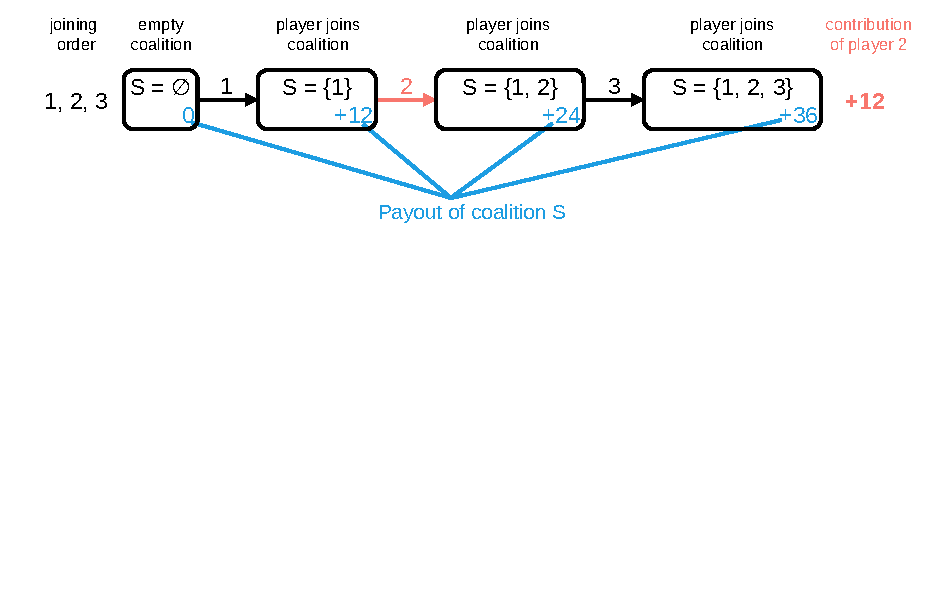
\includegraphics[page=1, width=0.8\textwidth]{figure/shapley_feature_effect}
  }
  \only<2>{
    \includegraphics[page=2, width=0.8\textwidth]{figure/shapley_feature_effect}
  }
\end{center}

\end{frame}


\begin{frame}{Proof of Axioms}
  The Shapley values fulfills all the 4 axioms.
  Symmetry, Dummy and Additivity relatively easy to proof:
\begin{itemize}
    % See also: https://math.stackexchange.com/questions/2747088/shapley-value-is-efficient
  \item \textbf{Symmetry}: Let's assume coalition $S \subseteq P - \{j,k\}$ and $v(S \cup \{j\}) = v(S \cup \{k\})$. 
    \begin{itemize}
        \item Then all marginal contributions are equal: $v(S \cup \{j\}) -  v(S) = v(S \cup \{k\}) -  v(S), \forall S \subseteq P - \{j,k\}$
        \item Consequently, $\phi_j = \phi_k$.
    \end{itemize}
  \pause
  \item \textbf{Dummy}: Let's assume we have Player $j$ such that for all $S \subseteq P$, we have $v(S) = v(S \cup \{j\})$. Then, each marginal contribution of player $j$ is zero, and therefore $\phi_j = 0$.
  \pause
  \item \textbf{Additivity}:  Assume two games $v_1$ and $v_2$ and a third game which is the sum of both $v(S) = v_1(S) + v_2(S)$. The marginal contribution for all $S \subseteq P - \{j\}$ for game $v$ can be expressed as $v(S \cup \{j\}) - v(S) = v_1(S \cup \{j\}) - v_1(S) + v_2(S \cup \{j\}) - v_2(S)$. Since the Shapley value is additive in the marginal contributions, we can split the sum into two sums so that $\phi_{j,v} = \phi_{j, v_1} + \phi_{j,v_2}$.
\end{itemize}
\end{frame}

\begin{frame}{Proof of Axioms (cont'd)}
    
Efficiency requires a bit more effort; proof sketch:
  \begin{itemize}
  \item \textbf{Efficiency}: $v(P)$ exactly appears once per player ($=p$ times) for coalition $S = P - \{j\}$ with the weight $\frac{|P - 1|!(|P| - |P - 1| - 1)!}{|P|!} = \frac{1}{p}$ each. The values for all other coalitions $v(S), S \subseteq P \{j,k\}$ appear with both minus and plus signs that cancel each other out.
\end{itemize}
\end{frame}


\begin{frame}{Linearity Axiom Corollary}
  \begin{itemize}
  \item The Shapley values are also linear:
  \item For a game with payout $v(S) = \alpha v_1(S) + v_2(S)$, the Shapley values are $\alpha \phi_{j,v_1} + \phi_{j,v_2}$.
  \item The multiplication with $\alpha$ works since we can pull out $\alpha$ from the sum of marginal contributions, so that for $v(S) = \alpha v_1(S)$ the Shapley value is $\alpha \phi_{j,v_1}$.
  \item We already know that Shapley values are additive which proofs the linearity.
  \end{itemize}
\end{frame}



\begin{frame}{Applications of Shapley Value}

  \begin{itemize}
      \item Game theory
      \item Economics (e.g., cost allocation) \lit{Moulin. 1992}{https://www.jstor.org/stable/2951524}
      \item Marketing (e.g., social network analysis to discover influencers) \lit{Naraynam et al. 2010}{https://ieeexplore.ieee.org/document/5499450}
      \item ...
      \item Machine learning
       \begin{itemize}
         \item Feature selection: Attribute loss reduction to features. \lit{Cohen et al. 2005}{https://www.ijcai.org/Proceedings/05/Papers/0763.pdf}
         \item Quantify data value: Attribute loss reduction to data points. \lit{Ghorbani et al. 2019}{https://arxiv.org/abs/1904.02868}
         \item Algorithm Selection: Attribute loss reduction to algorithms of portfolios. \lit{Fréchette et al. 2016}{https://www.aaai.org/ocs/index.php/AAAI/AAAI16/paper/view/12495}
         \item \alert{Explain individual predictions} $\leadsto$ local explanation.
       \end{itemize}
  \end{itemize}

\end{frame}



\end{document}
